\documentclass[dvipdfmx,tikz]{standalone}
\usepackage{tikz}
\usepackage{ifthen}
\begin{document}
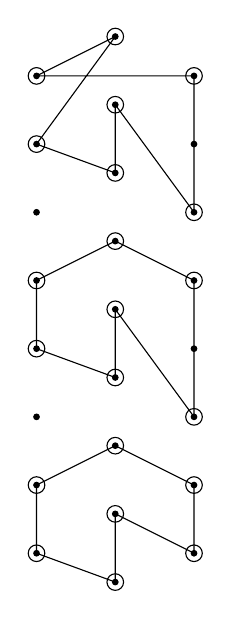
\begin{tikzpicture}
  \foreach \x in {0,...,2}{
      \pgfmathsetmacro{\range}{ifthenelse(mod(\x,2)==1,8,7)}
      \foreach \y in {0,...,\range}{
          \pgfmathsetmacro\shift{mod(\x,2)*0.5}
          \coordinate (a\x\y) at (\x, {-sqrt(3)/2*\y + \shift});
        }}
  \foreach \x in {0,...,2}{
      \pgfmathsetmacro{\range}{ifthenelse(mod(\x,2)==1,8,7)}
      \foreach \y in {0,...,\range}{
          \filldraw[draw=black,fill=black] (a\x\y) circle (1pt);
        }
    }

  \draw (a00) circle (3pt);
  \draw (a10) circle (3pt);
  \draw (a01) circle (3pt);
  \draw (a12) circle (3pt);
  \draw (a11) circle (3pt);
  \draw (a22) circle (3pt);
  \draw (a20) circle (3pt);
  \draw (a00) -- (a10) -- (a01) -- (a12) -- (a11) -- (a22) -- (a20) -- (a00);

  \draw (a13) circle (3pt);
  \draw (a03) circle (3pt);
  \draw (a04) circle (3pt);
  \draw (a15) circle (3pt);
  \draw (a14) circle (3pt);
  \draw (a25) circle (3pt);
  \draw (a23) circle (3pt);
  \draw (a13) -- (a03) -- (a04) -- (a15) -- (a14) -- (a25) -- (a23) -- (a13);

  \draw (a16) circle (3pt);
  \draw (a06) circle (3pt);
  \draw (a07) circle (3pt);
  \draw (a18) circle (3pt);
  \draw (a17) circle (3pt);
  \draw (a27) circle (3pt);
  \draw (a26) circle (3pt);
  \draw (a16) -- (a06) -- (a07) -- (a18) -- (a17) -- (a27) -- (a26) -- (a16);
\end{tikzpicture}
\end{document}
